\section{Scalable aggregation at line rate}
\label{sec:aggregation}
 High-speed routers typically feature an ingress and egress pipeline shared
across multiple ports, running at a 1 GHz clock rate to support up to a billion
64-Byte
packets per second of aggregate capacity (\S\ref{s:absmachine}).  To handle state updates
from packets arriving at 1 GHz, the key-value store for aggregations must be
available in SRAM on the router ASIC.  However, SRAM on an ASIC is limited,
restricting the size of an on-chip key-value store to a few Mbits (10K flows).

In principle, we could scale to a larger number of flows by making the on-chip
key-value store a cache for a larger off-chip store. In traditional cache
designs, cache misses require accessing off-chip DRAM with non-deterministic
latencies~\cite{unpredictable_cache} to read off the stored state. Because the
aggregation operation requires the value just read out from DRAM in order to update it
in the cache, the
entire operation incurs
non-deterministic latencies. This results in stalls in the router
pipeline. Unfortunately, pipeline stalls affect the router's ability to provide
guarantees on line rate packet processing (10-100G) on all ports.
%% Router pipelines are designed for the worst-case: they support line
%% rate (10 G or 100 G) on all ports at close to the smallest packet size. Pipeline
%% stalls can affect the router pipeline's ability to provide such worst-case
%% guarantees.\footnote{One could question this worst-case mindset, but we take it
%%   as a given because it obviates the need for performance profiling and has been
%%   the predominant design for the fastest routers for many years.}

\begin{figure}
\centering
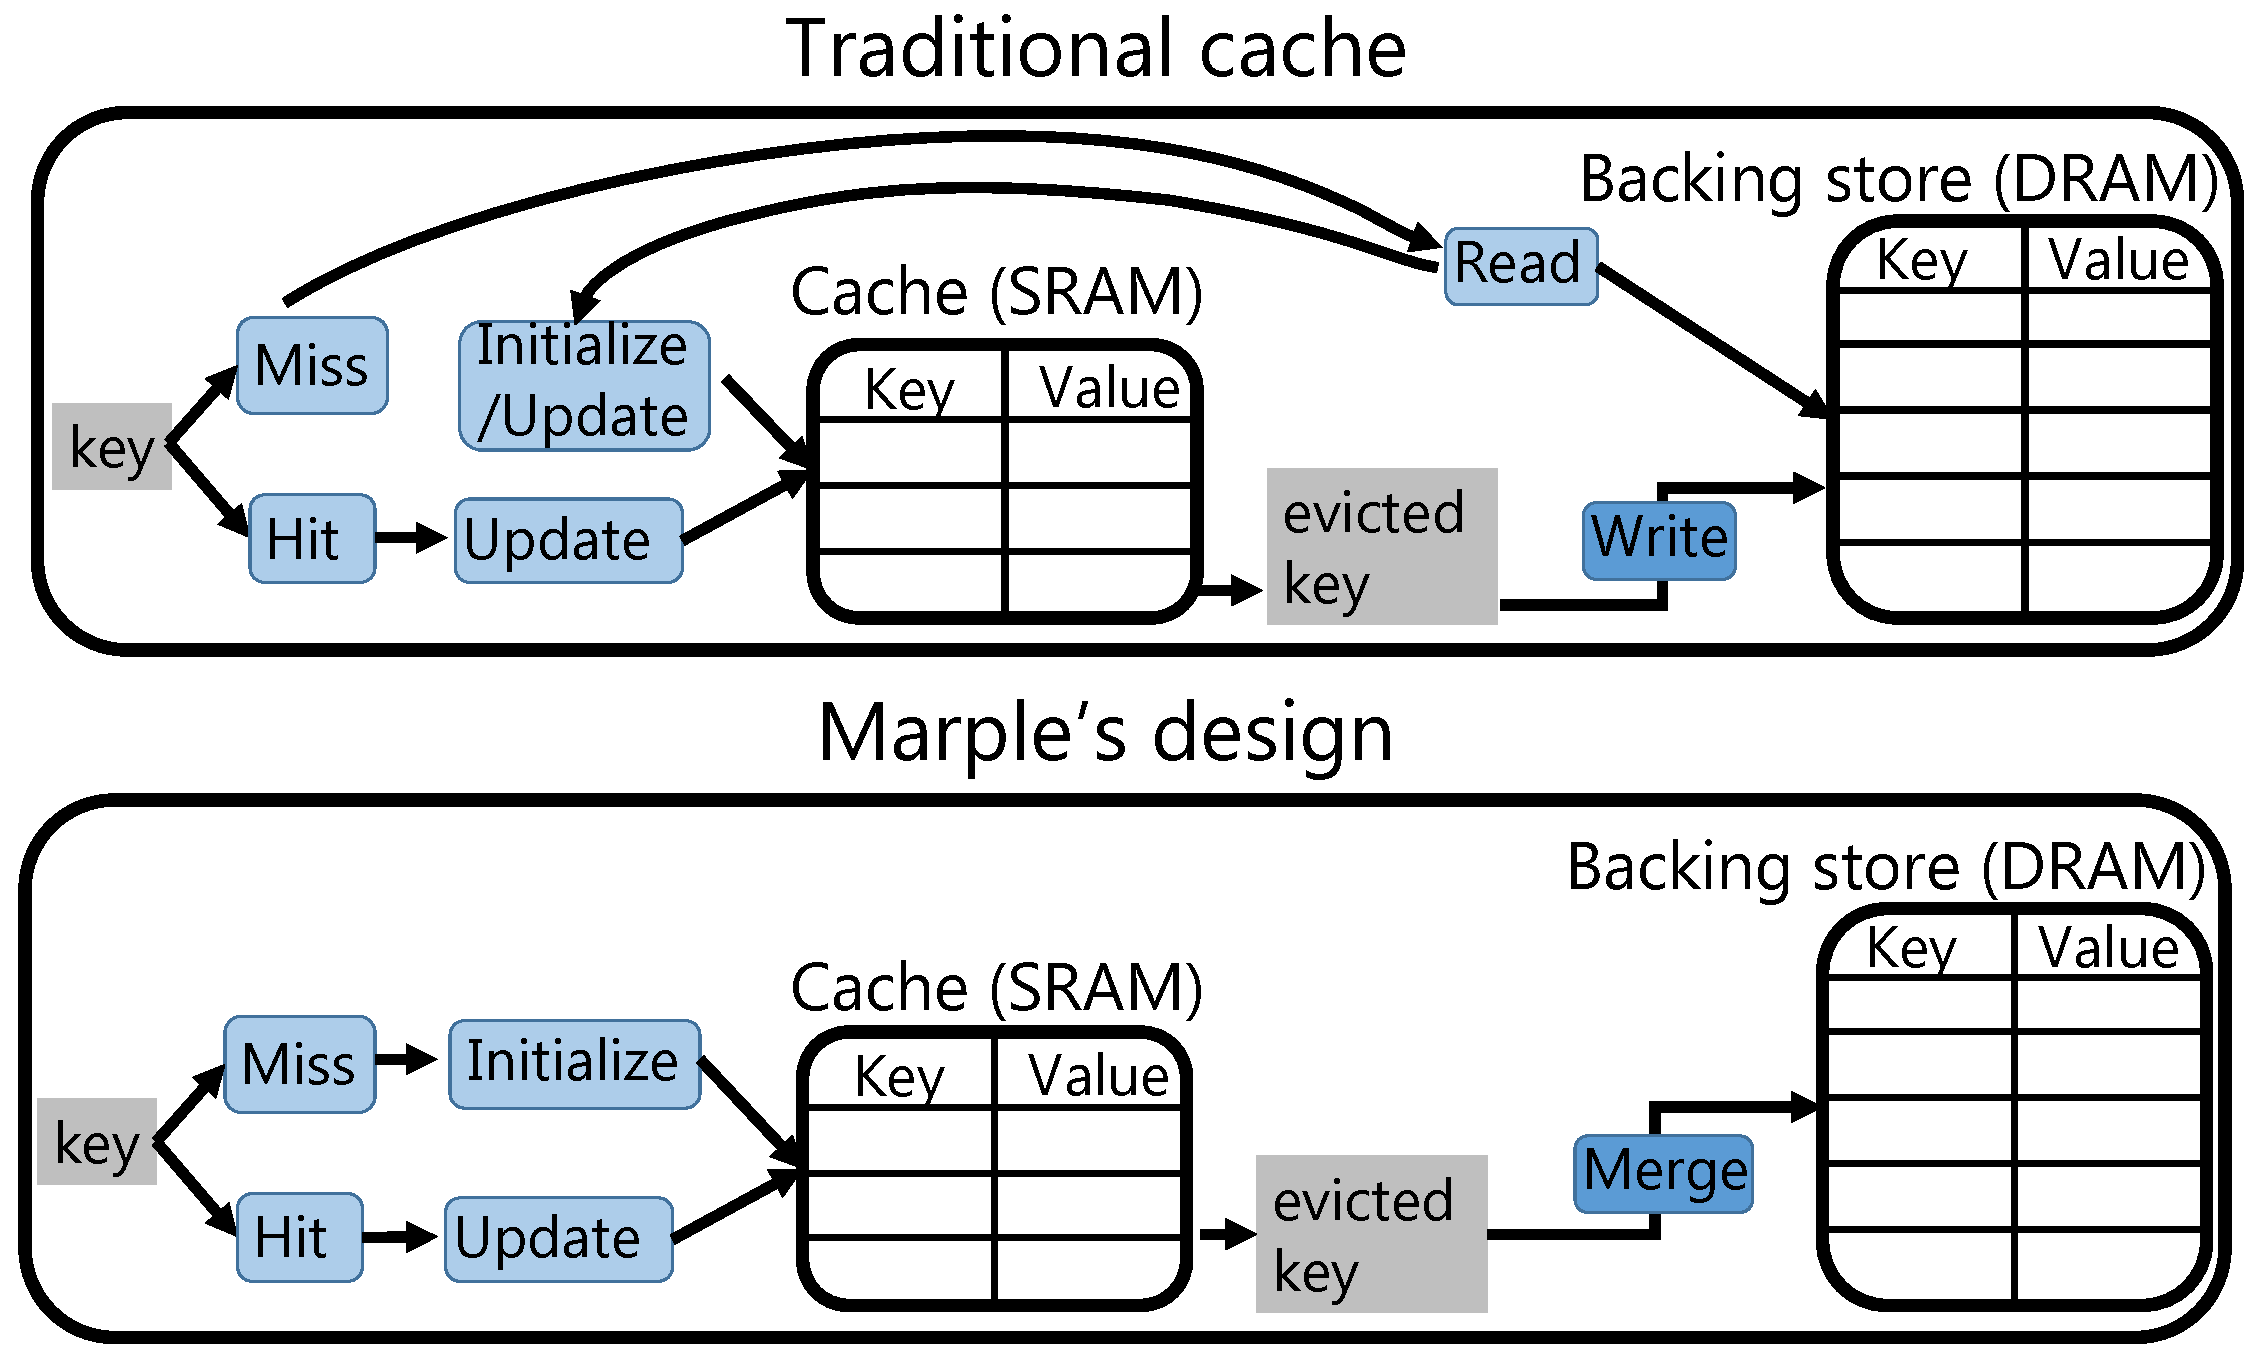
\includegraphics[width=0.6\columnwidth]{pq_kv_store.pdf}
\caption{\TheSystem's key-value store vs. a traditional cache}
\label{fig:kv}
\end{figure}

We design a key-value store that processes packets at line rate even on cache
misses (\Fig{kv}). Instead of stalling the pipeline waiting for a result from DRAM,
%% Normally, such misses result in a pipeline stall for
%% the time that it takes to fetch the missed packet's flow from memory.  Instead,
we treat the incoming packet as the first packet from a new flow and initialize
the flow's state to a default value. Subsequent packets from this flow are
aggregated within that flow's entry in the key-value store, until the flow is
evicted. When it is evicted, we {\em merge} the flow's value in the cache with
its value in the backing-store using a {\em merge function}, and write the
merged result to the backing store. The backing store may be stale relative to
the on-chip cache if there have been no recent evictions. We remedy this by
forcing periodic evictions.

But does merging guarantee correctness? For example, if an aggregation function
counts every flow's packets, the merge function could simply could add up the
cached and backed-up flow counts.
%% It is natural to ask if it is always possible to merge flow values and
%% guarantee correctness.
We characterize conditions that make aggregation functions accurately
``mergeable.''

\subsection{The associative condition}
A simple class of mergeable aggregation functions are associative
functions. For instance, suppose the aggregation function on state $s$ is $s =
op(s, f)$,
where $op$ is an associative operation and $f$ is a packet field. Then, if $op$
has an identity element $I$ and a flow's default value on insertion is $s_0 =
I$, it is easy to show that this function can be merged using the function
$op(s_{d}, s_{new})$, where $s_d$ and $s_{new}$ are the values in the backing
store and the cache, respectively. The associative condition allows us to merge
aggregation
functions like addition, max, min, set union, and set intersection.

\subsection{The linear-in-state condition}
\label{sec:linear-in-state-description}

Consider the example of the EWMA aggregation function, which maintains a moving
average of queueing latencies across all packets within a flow. The aggregation
function updates the EWMA $s$ as follows:
\[ s = (1 - \alpha) \cdot s + \alpha \cdot (t_{out} - t_{in}) \]
%TODO: Vikram: Can you check our simple algebra?
%TODO: Be consistent about flow or key
We assume $s$ is initialized to $s_0$ for all flows. Let us assume a flow $F$ is
evicted from the on-chip cache for the first time and written to the backing
store with an EWMA of $s_d$.\footnote{When a flow is first evicted, the merge
operation is trivial: we simply write the flow's current value into the backing
store.} The first packet from $F$ after $F$'s first eviction  is processed like a
packet from a new flow in the on-chip cache, starting with the state $s_0$.
Assume that $N$ packets from $F$ hit the on-chip cache after $F$'s first eviction,
resulting in the EWMA going from $s_0$ to $s_{new}$.  Then, the correct EWMA
$s_{correct}$ satisfies:
\begin{align*}
s_{correct} - (1-\alpha)^N s_d &= s_{new} - (1-\alpha)^N s_0 \\
s_{correct} &= s_{new} + (1-\alpha)^N(s_d - s_0)
\end{align*}

So, the correct EWMA can be obtained by: (1) having the on-chip cache store the
value $(1-\alpha)^N$ for each flow after each update, and (2) adding
$(1-\alpha)^N(s_d - s_0)$ to $s_{new}$ when merging $s_{new}$ with $s_d$. We
can generalize this example to show that we can merge any aggregation function
of the form $\boldsymbol{S} = \boldsymbol{A} \cdot \boldsymbol{S} +
\boldsymbol{B}$, where $\boldsymbol{S}$ is a vector of states, $\boldsymbol{A}$
and $\boldsymbol{B}$ are matrices whose entries are functions of the last $k$
packets, for some $k$ that can be determined at compile time. We call this
condition the {\em linear-in-state} condition, and we say that $A$ and $B$ are
functions of {\em bounded packet history}.
%TODO: Vikram, consider this if you have time:
% Prove that S=S*A + B is mergeable in the TR as well.
%, \ie put in the merge function for the general linear-in-state operation
% for matrices.

A {\ct groupby} with no {\ct emit}s and a linear-in-state (or associative)
aggregation function can be implemented scalably without losing accuracy because
it can be merged accurately.
However, if the {\ct groupby} uses an {\ct emit()} to pass tuples to another
query, it cannot be implemented scalably. An {\ct emit()} outputs the current state
of the aggregation function, for which the current state must always be
available in the router's on-chip cache. This is only possible if flows are
never evicted, effectively shrinking the key-value store to its on-chip cache
alone.

\subsection{Handling non-scalable aggregations}
\label{sec:workaround-nonscalable}
While the linear-in-state and associative conditions capture several aggregation
functions, and enable a scalable implementation, there are two practical classes
of queries that do not scale: (1) queries with aggregations
functions that are neither associative nor linear-in-state, and (2) queries where
the groupby has an {\ct emit} statement.

An example of the first class is the TCP non-monotonic query from
Figure~\ref{fig:example-perf-queries}, which counts the number of packets
with sequence numbers smaller than the maximum sequence number so far. It is
easy to see that {\ct nonmt} is not associative. It is not linear-in-state
either: the update can be rewritten as:
\\
%
{\ct count = count + (maxseq > tcpseq) ? 1 : 0}\\
%
While the update superficially resembles $\boldsymbol{A}
\cdot \boldsymbol{S} + \boldsymbol{B}$, the coefficient $\boldsymbol{B}$ is a
function of {\ct maxseq}, \ie the maximum sequence number so far, which
could be arbitrarily far back in the stream.
$\boldsymbol{B}$ is not a function of bounded packet history.

An example of the second class is the flowlet histogram query from
Figure~\ref{fig:example-perf-queries}, where the first {\ct groubpy} emits
flowlet sizes, which are grouped into buckets by the second {\ct groupby}.

%TODO: NG: define relation or table in language and here.
%TODO: Put an emit in the loss-rate query. It's not there.
There are workarounds even if aggregations fall in one of the two
non-scalable classes. One is to 
rewrite queries to remove {\ct emit}s.
For instance, we can rewrite the loss rate query
(\Fig{example-perf-queries}) to independently record the per-flow
counts for dropped packets and total number of packets in an aggregation table, and
have an operator read both tables every time they need the loss rate. Each
table can be scaled,
but the implementation comes at a transient loss of accuracy
relative to precisely 
tracking the loss rate after every packet using a {\ct zip.}  Second, an
operator may be content
with flow values that are accurate for each time period between two evictions,
but not across evictions (\Fig{accuracy-time}). Third, an operator
may want to run a query to collect data until the on-chip cache fills up and
then stop data collection. Finally, if the number of keys is small enough to fit
in the cache, the system can provide fully accurate results without evicting any
keys.
%% it possible to run the query with full
%% accuracy without evicting any flows.
%TODO: Examples for third and fourth workaround.
%TODO: Put modified loss rate in examples if space permits?

\subsection{General conditions for mergeability}

Why are certain aggregation functions mergeable, while others are not? Is there
a general condition that separates mergeable functions from non-mergeable ones?

%Anirudh->Vikram: removed logarithmic. It's too technical.
The answer is yes.
We state our results in the form of several theorems without proof. The proofs
are in Appendix~\ref{s:app:merge}.
Let $n$ denote the allowable size for state tracked in a \TheSystem query: it must be constant
and should not increase with the number of packets.
%Let $N$ be the number of
%packets seen between evictions of a particular key.
%Let $S$ denote the allowable state tracked in a stateful Marple query. It's only restriction is that
%the number of bits $n$ in this state is a small, at most logarithmic in $N$. Likewise, let $P$
%denote the header fields contained within the bounded packet history (this is a bounded constant number of bits).
%An \emph{aggregation function} is any function with signature $S \times P \rightarrow S$, essentially a fold function.
When merging state $s$ in the on-chip cache with state $s_d$ in the
backing store, the router may
need to maintain and send auxiliary state $a$ for the backing store to perform
the merge correctly. For example, in the EWMA example, the value $(1-\alpha)^N$
is auxiliary state. Then, a \emph{merge function} $m$ for an aggregation
function $g$ is a function
satisfying:
\[ m((s, a), s_d) = g(s_d, \{p_1, \ldots, p_N\}) \]
for any $N$ and sequence of packets $p_1, \ldots, p_N$. The application of $g$ to
a list of packets is shorthand for folding $g$ over each packet in order.

%% Does a merge function $m$ exist for every possible aggregation function $g$?
%% We now tackle the question: is there a general condition that separates mergeable and non-mergeable
%% functions? Our analysis of this question takes the form of several theorems, which are stated
%% here but proven separately in~\cite{theory-tr}. 
First, we show that \emph{every} aggregation function has a merge function, provided it's allowed to use
a large amount of auxiliary data.
%%\vspace{-0.18in}
\begin{theorem}
Every aggregation function has a corresponding merge function that uses
$O(n2^n)$ auxiliary bits.
\end{theorem}
%ANirudh->Vikram: need to justify why it can support only O(n) bits
Unfortunately, the on-chip cache supports only $O(n)$ bits of state: memory is limited
and \TheSystem shouldn't use much more state than indicated by the user's aggregation function.
We say an aggregation function
is \emph{mergeable} if the auxiliary state has size $O(n)$ for any arbitrary sequence of packets.
This characterization is consistent with what we
have described so far: the linear and associative conditions are indeed mergeable by this definition,
while queries that we cannot merge (\eg TCP non-monotonic in
\Fig{example-perf-queries}) violate it.
\begin{theorem}
If an aggregation function is either linear-in-state or associative, it has a merge function
that uses $O(n)$ bits of auxiliary state.
\end{theorem}
\begin{theorem}
The TCP non-monotonic query from \Fig{example-perf-queries} requires $\Theta(n2^n)$ auxiliary bits
in the worst case.
\end{theorem}
This begs the question: can we determine whether an aggregation function
is mergeable with $O(n)$ auxiliary bits? The answer is yes, but not easily.
\begin{theorem}
There exists an algorithm that computes the minimal number of auxiliary bits needed to merge a
given aggregation function.
\end{theorem}
The algorithm we construct is intractable, but it is unlikely that we can do much
better.
\begin{theorem}
Determining whether a merge function successfully merges an aggregation function
is co-NP-hard.
\end{theorem}
Hence, no polynomial time algorithm exists unless P=NP. 

%TODO: Make sure notation here is consistent with that in the appendix.
%SK->NG: Talk about stateless computations in the compiler.

\subsection{Hardware feasibility}
\label{sec:hardware-feasibility}
%TODO: Don't use the term entry
We optimize our stateful hardware design for linear-in-state queries and break
it down into five components.  Each component is well-known and our main
contribution is in putting them together to implement stateful queries.
Overall, the primary design choice for a router designer is how much memory to
provision for the on-chip cache, which we evaluate in \Sec{eval}. We now
discuss each component in detail.
%Figure~\ref{fig:pipeline} shows where each components is located within a router pipeline.
%TODO: add figure if space permits.

\textbf{The on-chip cache} is a hash table where each row in the hash table
stores keys and values for a certain number of flows. If a packet from a new
flow hashes into a row that is full, the least recently used flow within that row is
evicted. Each row has 8 flows and each flow stores 128 bits of key and 32 bits
of value.\footnote{The LRU policy is actually implemented across 3-bit pointers
that point to the keys and values in a separate memory. So we 
shuffle only the 3-bit pointers for the LRU, not the entire key and
value.} Our choice of 8 flows is based on 8-way L1 caches, which are very
common in processors~\cite{intel_opt_manual}. This cache eviction policy is
close to an ideal but impractical policy that evicts the least recently used
(LRU) flow across the whole table (\Sec{eval}).
%
Within a router pipeline stage, the on-chip cache has a logical interface
similar to an exact-match match-action table: namely, each packet matches into
the table using a key extracted from the packet header, and the corresponding
action is executed by the router.
%
%In addition, the cache adds and removes entries using the LRU policy.
%% piggybacking evicted entries on the packet itself.
%
Because of their similar interfaces, an on-router hash table can be used as
a path to
incremental deployment.
%% Within a router pipeline stage,
%% the on-chip cache has the same wiring interface to the remaining pipeline stages as a
%% traditional match-action table.
%TODO: Anirudh. Last sentence is a bit vague. Not sure how to fix it.

\textbf{The off-chip backing store} is a scale-out key-value store such as
Redis running on dedicated collection servers within the network. As
\Sec{eval} shows, the number of measurement servers required to support
typical eviction rates from the router's on-chip cache is small.%%  fraction of
%%  the cost
%% of the network.
%TODO: Remove this if eval does not show this.

\textbf{Maintaining packet history.} Before a packet reaches the pipeline stage
with the on-chip cache, we use the preceding stages to precompute
$\boldsymbol{A}$ and $\boldsymbol{B}$ (the functions of bounded packet history)
in the state-update operation $\boldsymbol{S} =\boldsymbol{A} \cdot
\boldsymbol{S} + \boldsymbol{B}$. Our current design only handles the case
where $\boldsymbol{S}$, $\boldsymbol{A}$, and $\boldsymbol{B}$ are scalars. Say
$\boldsymbol{A}$ and $\boldsymbol{B}$ depend on packet fields from the last $k$
packets. Then, these preceding pipeline stages act like a shift register and
store fields from the last $k$ packets. Each stage contains a read/write
register, which is read by a packet arriving at that stage, then carried with
the packet, and finally written into the next stage. Once values from the last
$k$ packets have been read into packet fields, $\boldsymbol{A}$ and
$\boldsymbol{B}$ can be computed using the stateless instructions provided by
programmable router architectures (\cite{rmt} and Chapter~\ref{chap:domino}).

\textbf{Carrying out the linear-in-state operation.} Once $\boldsymbol{A}$ and
$\boldsymbol{B}$ are known, we use a multiply-and-accumulate (MAC)
instruction~\cite{mac} to compute $\boldsymbol{A} \cdot \boldsymbol{S} +
\boldsymbol{B}$. 
This instruction is very cheap to implement: our circuit synthesis experiments
show that a MAC instruction meets timing at 1 GHz and occupies about 2000
\si{\micro\metre\squared} in a recent 32-nm transistor library. A router
chip with an area of a few hundred \si{\milli\meter\squared} can easily support
a few hundred MAC instructions.

\textbf{Queries that are not linear-in-state.} We use the set of stateful
instructions developed in Domino (Chapter~\ref{chap:domino}) for queries that are not
linear-in-state. Our evaluations show that these instructions are sufficient
for our non linear-in-state queries.
%TODO: Reconfig. in LRU? Maybe this is not even required ...

%We leave the question of
%designing hardware for multi-pipeline routers to future work.

%TODO: Domino doesn't implement the entirety of the hardware design.  Maybe I
%should do that to round out the store and say we have implemented the hardware
%design in a C++ simulator. I think it will involve implementing the LRU, which
%shouldn't be too hard.

%TODO: Define data-plane program, on-chip cache etc. Be consistent.
